\chapter{Data Collection}
This chapter details the data collection process for the building blocks of the social network. It begins by explaining the origin of the data collection strategy, and then describes the data sources, research database schema, and domain constraints, followed by an explanation of the data collection algorithm.

\section{Initial Research Question and Data Collection}

This research project originally began with a different goal: the intent was to identify differences in commit behavior between paid and volunteer contributors of open source projects. However, due to challenges in data collection, the project was changed to analyze organizational networks instead. This section provides some context on why this decision was made, and how it shaped the direction of the data collection.

The primary experimental task in the original project was to classify contributors as paid or volunteer so that the differences in commit behavior between these classes could be evaluated. A script was written which collected data from Git, Github, and JIRA profiles of ASF contributors and used several heuristics to perform the classification. 
However, two issues made it difficult to identify the differences between the two classes:
\begin{enumerate}
	\item \label{manypaid} For a given ASF project and time period, the proportion of active contributors who are paid to work on the project can be very high, sometimes nearing 100\%.
	\item \label{novolunteers} A profile can contain certain markers that are highly correlated with paid contributors, but there are no known markers that are highly correlated with volunteer contributors.
\end{enumerate}
Issue \#\ref{manypaid} was \emph{prima facie} quite surprising---one might expect there to be a somewhat even mix of paid and volunteer contributors, but upon manually examining contributors to a couple projects, it was discovered that these projects were almost exclusively developed by employees of a few companies during the time period under observation. With such skewed samples, it became difficult to write a classifier sensitive enough to be useful.
Issue \#\ref{novolunteers} was an unforeseen limitation of using profile information to identify social group affiliation. Ultimately, there was no reliable way to differentiate between a volunteer and a paid contributor when his/her data does not reveal any obvious link between his/her contributions and his/her employer.

Since creating this classifier proved infeasible, the data was re-purposed to do a social network analysis of ASF contributions instead. 
The Git, Github, and JIRA data was general enough to be applicable to the new research direction. In particular, the following facets of the existing dataset were useful:
\begin{itemize}
	\item For any given contributor, the dataset typically contained data from multiple accounts/profiles, which improved the reliability of finding a given contributor's employer.
	\item Since the contributor's employer name was necessary for one of the heuristics, a fair amount of employer data was already available.
\end{itemize}
In addition, since the dataset included information about JIRA contributions, these contributions were also considered (alongside commits) when creating edges in the social network. This revealed organizational connections that would not have appeared when considering commits alone.

\section{Data Sources}

In order to identify the employers of the project contributors, the script attempts to collect relevant data from Git, JIRA, and Github accounts. It also utilizes the Google Custom Search API to find links to contributors' LinkedIn profiles, which can then be inspected manually. Each of these sets of values is stored in a separate entry in a relational database, to maximize the amount of information available for finding a contributor's employer.
The following information is mined from Git, Github, and JIRA accounts:
\begin{itemize}
	\item Email address
	\item Display name
\end{itemize}
The following additional information is mined from Git logs:
\begin{itemize}
	\item Number of commits authored by each account during \timeperiod{}
\end{itemize}
The following additional information is mined from Github accounts:
\begin{itemize}
	\item Username
	\item Location
	\item Company name
	\item List of organizations
\end{itemize}
The following additional information is mined from JIRAs:
\begin{itemize}
	\item Username
	\item Number of issues created or resolved by each account during \timeperiod{}
\end{itemize}
In addition, to work around the rate limits of the Github API, the script utilized an offline GHTorrent database dump as a cache of Github account data. GHTorrent is a repository containing terabytes of Github data, developed by Georgios Gousios to aid software repository research\cite{Gousi13}.

\pddone{Add a section here between 2.2 and 2.3, entitled "Schema of Mined Data" explaining the schema of all your data, viz., all relations,  including accountprojects} \bmdone{Created section ``Database Schema'', please review.}

\section{Database Schema}
All the collected data was stored in a set of relational databases. Due to technical limitations in some of the project's external dependencies (explained below), multiple different databases were required. The following subsections describe the purpose and schema of each database. In the schema diagrams, foreign keys are denoted with an asterisk.
\subsection{GHTorrent Database}
A MySQL dump of the 2016 GHTorrent database was downloaded from GHTorrent.org and installed locally. This database was used as a ``proxy cache'' for the live Github data, providing unrestricted access to most of the necessary Github data. This resulted in a significant performance improvement, compared to exclusively using the Github API, which has a restrictive rate limit that would have bottlenecked the data collection. The relevant portion of the schema is shown in figure \ref{fig:ghtorrentSchema}.
\begin{figure}
	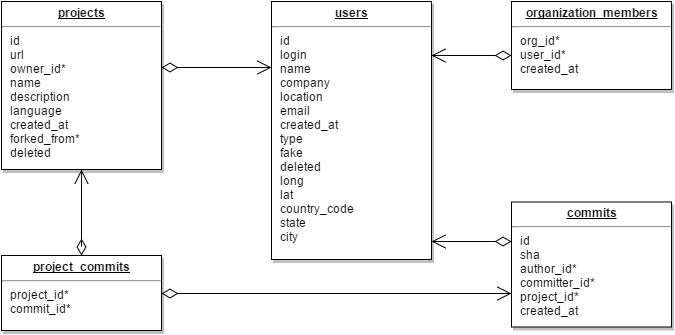
\includegraphics[width=\textwidth]{GHTorrentSchema.png}
	\centering
	\caption{The relevant tables of the GHTorrent database}
	\label{fig:ghtorrentSchema}
\end{figure}
\subsection{CVSAnalY2 Databases}
The CVSAnalY2 tool\cite{cvsanaly} was used to parse each project's Git log data and transform it into a database that could be analyzed more quickly and conveniently. At the time of writing, CVSAnalY2 only supports MySQL databases. One database was created for each project analyzed, with the name \verb|<<project_name>>_git|. The relevant portion of the schema of these databases is shown in figure \ref{fig:cvsanalySchema}.
\begin{figure}
	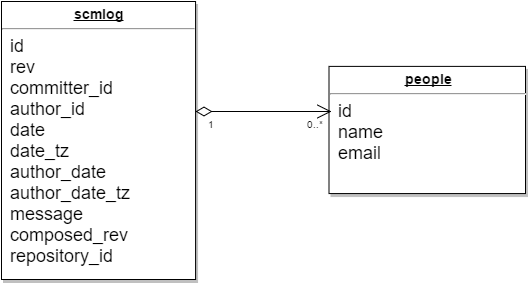
\includegraphics[scale=0.8]{cvsanalySchema.png}
	\centering
	\caption{The relevant tables of each CVSAnalY2 database}
	\label{fig:cvsanalySchema}
\end{figure}
\subsection{Main Database}
The main research database contains all the data collected from Git, Github, and JIRA, and all data derived thereof. It is stored in PostgreSQL\footnote{At the time when the database was created, there was not yet a dependency on CVSAnalY2 or GHTorrent, so it was created in PostgreSQL. By the point when it became clear that the dependencies required MySQL, the cost of porting the existing code to use it outweighed the benefits of using a single DBMS, so the main database remained in PostgreSQL. Since the databases were generally accessed through the SQLAlchemy ORM abstraction layer anyway, this was not too much of an inconvenience.}. The data in this database is used to build the \textbf{contributorprojectcommitcount} table, which is then imported into R for social network analysis.

The primary tables for the data collection are \textbf{contributors} and \textbf{contributoraccounts}. \textbf{contributoraccounts} stores the data for each Git, Github, and JIRA account. Each row has a foreign key to \textbf{contributors}, which allows the association of multiple accounts to a single person. The table \textbf{emailprojectcommitcount} maps an email address found in \textbf{accountprojects} to the number of commits that account authored for each project. With these three tables, we derive \textbf{contributorprojectcommitcount}. The table \textbf{contributorcompanies} maps a contributor to their employer. The generation of this table is discussed in section \ref{employersec}. Joining \textbf{contributorcompanies} and \textbf{contributorprojectcommitcount} creates \textbf{companyprojectcommitcount}, which is then used as the basis of generating the organizational social networks. The schema for this database is shown in figure \ref{fig:mainSchema}.
% TODO: decide if necessary to include accountprojects
\begin{figure}
	\includegraphics[width=\textwidth]{mainSchema.png}
	\centering
	\caption{The schema of the main research database}
	\label{fig:mainSchema}
\end{figure}

\section{Data Collection Constraints}
Building a social network of employers from contribution artifacts was not trivial, because employment is a social abstraction, as opposed to a value that can be directly extracted from these artifacts. In order to make this project feasible, a few constraints needed to be placed upon the scope of the data collection.

One specific issue with the data collection was that since a contributor's employer name can only be obtained if the contributor chooses to reveal it, there will typically be some individuals for whom no employer name could be found. Furthermore, this information must be mined automatically for the majority of contributors, or else it becomes infeasible to manually fill in all the missing values. After performing some trial experiments, it was found that achieving high employer identification rates can be very challenging on larger projects such as Apache Kafka, which have many individual contributors. 
However, it was still possible to accurately measure organizational contributions, for the following reason: through experimentation it was found that the vast majority of commits to a project typically came from a small subset of the committers; since these contributors were the most active, it was sufficient to identify only their employers and ignore the others, without damaging the validity of the results. For this reason, the data collection was limited to only the prolific contributors of each project, defined as contributors in the minimum size set S such that the sum of the number of commits done by members of S during \timeperiod{} is at least 80\% of the number of commits done to the project. This also had the effect of improving the proportion of employer names mined automatically, because prolific contributors seem to be more likely to keep their Git, Github, and JIRA profile information up-to-date.

An additional constraint was that only ASF projects which met the following conditions were considered:
\begin{enumerate}
	\item \label{ghtreq} The project is listed in the GHTorrent database
	\item \label{jirareq} The project has a JIRA hosted at \ASFJIRAURL
	\item \label{commitreq} At least 20 commits were done to the project within the period under observation
\end{enumerate}
In general, these constraints resulted in the exclusion of projects which lacked sufficient data to analyze. \#\ref{ghtreq} allowed selection of projects that were hosted on Github. \#\ref{jirareq} ensured each project had a JIRA that could be automatically mined for additional account information. \#\ref{commitreq} excluded projects with few commits, because they would have added noise to the social networks, in the form of highly insignificant edges. The final set of projects mined is shown in table \ref{tab:projectcommitcounts}.

\begin{table}
	\begin{tabular}{l|c}%
		\bfseries Project & \bfseries Commits in Period% specify table head
		\csvreader[head to column names]{projectcommitcounts.csv}{}% use head of csv as column names
		{\\\hline\project & \sum}% specify your coloumns here
	\end{tabular}
	\begin{tabular}{l|c}%
		\bfseries Project & \bfseries Commits in Period% specify table head
		\csvreader[head to column names]{projectcommitcounts2.csv}{}% use head of csv as column names
		{\\\hline\project & \sum}% specify your coloumns here
	\end{tabular}
	\centering
	\caption{The ASF projects mined, with the number of commits authored in \timeperiod{}}\label{tab:projectcommitcounts}
\end{table}

\section{Data Collection Algorithm}
The script jiradb.py performs the majority of the data gathering. Its algorithm can be summarized as follows:
\begin{enumerate}
	\item Get JIRA account data for contributors to the JIRAs of the projects (See section \ref{jirasec})
	\item Get Git account and commit data for committers to the projects (See section \ref{gitsec})
	\item Get Github account data for Git accounts (See section \ref{githubsec})
	\item Associate accounts belonging to a single person under a single contributor ID (See section \ref{mergingsec})
	\item Generate a guess for the employer of each contributor (See section \ref{employersec})
\end{enumerate}

Each individual set of profile data is stored in a row of the \textbf{contributoraccounts} table of the research database. This table relates individual contributors to the accounts that they used to contribute. The following sections provide more details on the data collection steps.

\subsection{JIRA Data}\label{jirasec}
The JIRA Python package was used to query the ASF JIRA at \ASFJIRAURL. JIRA can be queried programatically by using the JIRA Query Language (JQL). The following JQL query was used to download issues for project \textbf{P} that were either created or resolved in \timeperiod{}:
\begin{lstlisting}
project = "P" AND created < "2016-06-01 00:00" AND (created >
 "2016-01-01 00:00" OR resolved < "2016-06-01 00:00")
\end{lstlisting}
After the issues were downloaded, each issue's metadata and history was processed to find JIRA accounts that either created or resolved the issue in \timeperiod{}. The profile information for each account was stored as an entry in \textbf{contributoraccounts}.
\subsection{Git Data}\label{gitsec}
The CVSAnalY2 tool was used to generate databases containing structured Git log data for each project. Each log database was queried to obtain the total number of commits authored in \timeperiod{}. If it was less than 20, the project was excluded from further analysis. Otherwise, each commit author's email address was cross-referenced against the GHTorrent database to find his/her Github account(s). For each Github account found, a row was inserted into \textbf{contributoraccounts} with the Git account's email adress and display name, and with the username column set to the Github account's username. Finally, if the email address had not been seen before, a row was added to table \textbf{emailprojectcommitcount} relating the address to the number of commits authored from that address to the project during \timeperiod{}.
\subsection{Github Data}\label{githubsec}
Whenever a new Git or JIRA account was processed, the account information was used to find the associated Github account. Matching against Git account information was typically more reliable than using JIRA, since Github users are encouraged to add their Git email address to their Github accounts. However, in cases where the user did not do so, sometimes they used their JIRA account's email address instead, so the accounts could be associated through that. The next section provides more detail on how this matching is done.

A given contributor in the \textbf{contributors} table may have multiple associated Github usernames through different matchings of Git and JIRA account information. Technically, Github allows an email address to be associated with only one Github account, but due to inaccuracies in the GHTorrent dataset, this constraint cannot be relied upon. To mitigate this problem, although a row in \textbf{contributoraccounts} is created for each possible Github username linked with a given email address in GHTorrent, the only direct usage of these usernames was for identity matching purposes. In cases where actual Github profile information was needed, the usernames were validated using the Github API before use, and the first valid one was taken as the contributor's official Github username.

Since one of the constraints placed on the mined projects was that the project was listed in GHTorrent, it was ensured that every project's Git repository was hosted (or at least mirrored) on Github. As a result, most of the contributors had a Github account. This was important because these accounts have several fields that help with employer identification, especially the ``company'' field, which is the only field in the dataset that can reveal an employer name directly.
\subsection{Identity Matching}\label{mergingsec}
Two accounts were considered to belong to the same person when at least one of the following was true:
\begin{itemize}
	\item The accounts use the same email address
	\item The accounts use the same username and service (i.e. Git or JIRA)
\end{itemize}
The only exception to these rules was that accounts which used the email address ``dev-null@apache.org'' were not paired based on the email alone, because this is a shared email address used by multiple ASF contributors. For the purpose of identity matching, Git and Github were considered to be the same service.

For each new contributor found (i.e. whenever a new account could not be associated with an existing account using the above rules), a row was added to the \textbf{contributors} table of the research database. Then, the new account information was used to query the GHTorrent database to find the associated Github account. Failing that, a similar query was performed against the live Github API. If the Github account was found, the login, company, and location values were stored in the newly created \textbf{contributors} row.

\subsection{Employer Identification}\label{employersec}
As explained earlier, it was not always possible to immediately pinpoint a contributor's employer with a high degree of confidence. However, it was usually possible to generate a number of guesses, 
based on the data contained in the contributor's accounts. Employer guesses were collected from account information, synthesized into a final guess for each contributor, and inspected and corrected manually.
Employer guesses were generated from the following sources:
\begin{itemize}
	\item ``Company'' field of Github profiles
	\item Domain name of email addresses
	\item Employment history in LinkedIn profiles
\end{itemize}
LinkedIn page URLs were found by using Google Custom Search API to search linkedin.com using the concatenation of each account's display name and the name of the project that account contributed to. These pages were then inspected manually, to verify the match was correct, and to find out which organization employed the profile owner most recently during \timeperiod{}. ``Apache Software Foundation'' was never recorded as the true employer, because ASF has no employees\cite{asf}.

Once these employer guesses were generated, a determination of each contributor's employer was made based on the following prioritization:
\begin{enumerate}
	\item If the employer name came from LinkedIn, it takes precedence over all other possibilities, because LinkedIn was usually the most up-to-date of the profiles, and employment history is an essential part of this profile.
	\item Otherwise, if the contributor's Github profile listed an employer, it was taken.
	\item If neither LinkedIn nor Github provided an employer guess, it was left for manual inspection.
\end{enumerate}
Additionally, any employer name that appeared only once in the dataset was also included in manual verification, based off the intuition that such values were more likely to be incorrect, as opposed to the alternative possibility, which is that the organization assigned only one person to the projects. Errors in employer identification could be caused by mistakes in identity matching, or out-of-date profile information, resulting in such anomalies.
The manual verification uncovered the true employers of all but six of the contributors whose employer name was missing or appearing once. Instead of excluding these contributors from further analysis, their employer names were set to \verb|Unknown <Unique_ID>|, effectively classifying them as independent volunteers. Of the 92 contributors with employer name appearing once, 42 were found to be incorrect, and subsequently corrected.

In the final step of data cleaning, different spellings and capitalizations of employer names were normalized by manually constructing a mapping table from each variant spelling to the most common spelling (in terms of how many of the contributors used it in their profiles.) The total number of unique organizations in the dataset, including the six unknown ones, was 93. The number of active contributors per organization is listed in table \ref{tab:orgcontributors} of appendix \ref{ch:orgdata}.